% uringpy-http: the paper. Build: latexmk -pdf paper.tex
% Two-column layout close to IEEEtran; with IEEEtran.cls available, the
% \documentclass line can be swapped for \documentclass[conference]{IEEEtran}.
\documentclass[10pt,twocolumn,letterpaper]{article}
\usepackage[T1]{fontenc}
\usepackage{mathptmx}
\usepackage[scaled=0.9]{helvet}
\usepackage{courier}
\usepackage[letterpaper,margin=0.72in,columnsep=0.22in,top=0.75in,bottom=0.9in]{geometry}
\usepackage{graphicx}
\usepackage{booktabs}
\usepackage{amsmath}
\usepackage{xcolor}
\usepackage{microtype}
\usepackage[hidelinks]{hyperref}
\usepackage{url}
\usepackage{titlesec}
\usepackage{caption}
\usepackage{enumitem}
\usepackage{tikz}
\usetikzlibrary{arrows.meta,positioning,fit,backgrounds}

\titleformat{\section}{\centering\normalsize\scshape}{\Roman{section}.}{0.5em}{}
\titleformat{\subsection}{\normalsize\itshape}{\Alph{subsection}.}{0.5em}{}
\titlespacing*{\section}{0pt}{1.4ex}{0.8ex}
\titlespacing*{\subsection}{0pt}{1.0ex}{0.5ex}
\captionsetup{font=footnotesize,labelfont=sc,labelsep=period}
\captionsetup[table]{position=top,justification=centering}
\setlist{nosep,leftmargin=1.2em}
\renewcommand{\thetable}{\Roman{table}}
\newcommand{\code}[1]{\texttt{#1}}
\newcommand{\kx}{$\times$}
\setlength{\tabcolsep}{3.2pt}

\title{\LARGE Parsing HTTP Outside the Lock: An \texttt{io\_uring} ASGI Server\\ with a C Parser and GIL Batching}
\author{Marimuthu Velayutham\thanks{M.~Velayutham is an independent researcher
(e-mail: marimuthu.vm@gmail.com; ORCID: 0009-0007-7352-5552).}}
\date{}

\begin{document}
\maketitle

\begin{abstract}
\noindent\textbf{\textit{Abstract}---A Python web server usually parses
HTTP while it holds the Global Interpreter Lock (GIL), and calls the
application once per request. We built \code{uringpy-http}, an ASGI server
whose \code{io\_uring} transport and HTTP/1.1 parser run in C with the GIL
released. The GIL is taken once per batch of requests, and each request
starts the application as an eager \code{asyncio} task. Unmodified Starlette
and FastAPI applications run on it. We compared it with Uvicorn and Granian
on a four-core cloud server in 694 runs with no failures, against
expectations recorded before the runs. With one worker, a request served by
\code{uringpy-http} costs much less than the same request through Uvicorn
with \code{httptools} and \code{uvloop}: throughput is 3.36\kx{} as high for
a raw ASGI app, 2.41\kx{} for Starlette and 1.47\kx{} for FastAPI. With four
worker processes the ratios are 2.76\kx{}, 2.14\kx{} and 1.44\kx{}. Granian's
are 1.32\kx{}, 1.29\kx{} and 0.91\kx{}. Batching the GIL doubles what four
worker threads of one interpreter deliver on the raw app (2.09\kx{}), and
cuts voluntary context switches from 1.1 to 0.02 per request. Still, it
reaches only 0.76 of four processes, short of the 0.90 we expected. Framework
code holds the GIL for 21\,\textmu s per request (Starlette) and
106\,\textmu s (FastAPI), so four threads stay under the ceiling of one over
that time; the threads then deliver 0.34 and 0.26 of processes. On the
free-threaded build the same threads reach 0.97 (raw) and 0.84 (FastAPI) of
processes. Code, raw data and scripts are public.}
\end{abstract}

\noindent\textbf{\textit{Index Terms}---io\_uring, ASGI, HTTP parsing,
Python, Global Interpreter Lock, web servers, free-threading}

\section{Introduction}

A request to a Python web application crosses three layers. The transport
moves bytes on and off the socket. The HTTP parser turns those bytes into a
method, a path and headers. The application turns the request into a
response. In the usual deployment, Uvicorn~\cite{uvicorn} with
\code{httptools} and \code{uvloop}~\cite{uvloop}, the parser is written in C
(llhttp~\cite{llhttp}). It still reports each part of the request through a
Python callback, though, and the event loop runs Python code for every read
and write. All of that holds the GIL, so the server's own work competes with
the application for one lock. That is why Python servers scale by running
one process per core.

Our earlier study~\cite{uringpy} measured what this costs for worker threads
that share one interpreter. It found that the number of times the GIL
changes hands matters more than the system-call interface. A reactor written
in C that takes the GIL once per batch of requests, rather than once per
request, brought four threads from 0.79\kx{} to 2.38\kx{} the throughput of
one. That study used a synchronous handler written for the benchmark and did
not parse HTTP. Its conclusion named the next step: a server that parses
HTTP in C and enters Python only to run the application.

This paper takes that step behind the standard interface, ASGI~\cite{asgi},
so that real frameworks run unchanged. We ask four questions.
\begin{enumerate}[label=Q\arabic*.]
\item How much does one request cost when the transport and the parser run
  outside the GIL, compared with Uvicorn and Granian?
\item Does GIL batching still help worker threads when the handler is an
  ASGI application, which builds a scope and steps a coroutine for each
  request?
\item How long does a real framework hold the GIL, and what does that time
  allow threads to deliver?
\item What changes on the free-threaded build?
\end{enumerate}

The paper makes three contributions. The first is \code{uringpy-http}, an
ASGI server on \code{io\_uring} with picohttpparser~\cite{picohttpparser}
running without the GIL. It takes the GIL once per batch of requests and
starts each application as an eager \code{asyncio} task (Section~III). The
second is a comparison with Uvicorn and Granian~\cite{granian} that covers
three applications, one to four workers, threads and processes, both CPython
builds and open-loop load, with expectations committed before the runs
(Sections~IV and~V). The third is a measurement of how long the GIL is held
per request inside Starlette and FastAPI, and of what that time limits
(Section~V-C).

\section{Background and Related Work}

\textbf{ASGI.} An ASGI application is an \code{async} callable
\code{app(scope, receive, send)}~\cite{asgi}. The server builds \code{scope},
a dictionary with the method, path, headers and other details of one
request. The application awaits \code{receive()} for the body and calls
\code{send()} twice, once with the status and headers and once with the
body. Starlette~\cite{starlette} and FastAPI~\cite{fastapi} are ASGI
frameworks. Uvicorn~\cite{uvicorn} and Hypercorn run ASGI applications on
\code{asyncio}, and Granian~\cite{granian} runs them on a Rust HTTP stack. In
production these servers scale with one process per core.

\textbf{Parsing.} \code{httptools} wraps llhttp~\cite{llhttp}, a C parser
that reports a request through callbacks; in Uvicorn each callback is a
Python method. h11 is written entirely in Python. picohttpparser
\cite{picohttpparser} parses a whole header block in one call, writes the
results into an array the caller provides, and uses SIMD instructions where
they are available; H2O~\cite{h2o} uses it. We use picohttpparser because a
single call with no callbacks can run with the GIL released.

\textbf{The GIL and \code{io\_uring}.} The GIL lets one thread run Python
code at a time. How badly it treats I/O-bound threads is known since
Beazley~\cite{beazley}, and the effect is an instance of Amdahl's
law~\cite{amdahl} for contended critical sections~\cite{eyerman}.
\code{io\_uring}~\cite{axboe} lets a program submit many I/O operations and
collect their completions with one system call. The earlier
study~\cite{uringpy} combined the two. With one Python call per request,
throughput is bounded by $X_N \le 1/(t_p + g\tau)$. Here $t_p$ is the time a
request holds the GIL, $g$ is the number of GIL hand-offs per request, and
$\tau$ is the cost of each hand-off. Batching lowers $g$; it cannot lower
$t_p$. PEP~703~\cite{pep703} made a build without the GIL available, and it
is supported from CPython~3.14.

\section{Design}

\code{uringpy-http} is about 1,500 lines of Cython and Python plus the
vendored picohttpparser and liburing~2.6. One \emph{engine} is one worker. It
owns an \code{io\_uring} ring, a listening socket with \code{SO\_REUSEPORT}
and a connection table indexed by file descriptor. Engines share nothing.
They run as threads of one interpreter or as one process each.
Figure~\ref{fig:pipeline} shows one pass over the completion queue.

\begin{figure}[t]
\centering
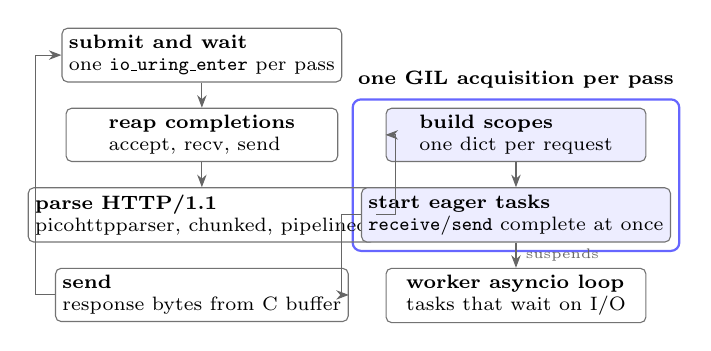
\begin{tikzpicture}[font=\scriptsize, node distance=3.2mm,
  box/.style={draw=black!55, rounded corners=2pt, minimum width=3.45cm, minimum height=6.4mm, align=left, inner sep=2.5pt},
  gilbox/.style={box, fill=blue!7},
  arr/.style={-{Stealth[length=1.6mm]}, black!60}]
\node[box] (sub) {\textbf{submit and wait}\\one \code{io\_uring\_enter} per pass};
\node[box, below=of sub] (reap) {\textbf{reap completions}\\accept, recv, send};
\node[box, below=of reap] (parse) {\textbf{parse HTTP/1.1}\\picohttpparser, chunked, pipelined};
\node[box, below=of parse] (ser) {\textbf{send}\\response bytes from C buffer};
\node[gilbox, right=6mm of reap, minimum width=3.3cm] (scope) {\textbf{build scopes}\\one dict per request};
\node[gilbox, below=of scope, minimum width=3.3cm] (run) {\textbf{start eager tasks}\\\code{receive}/\code{send} complete at once};
\node[box, below=of run, minimum width=3.3cm] (loop) {\textbf{worker asyncio loop}\\tasks that wait on I/O};
\begin{scope}[on background layer]
\node[draw=blue!60, thick, rounded corners=3pt, fit=(scope)(run), inner sep=3pt, label={[font=\scriptsize\bfseries]above:one GIL acquisition per pass}] (gil) {};
\end{scope}
\draw[arr] (sub) -- (reap);
\draw[arr] (reap) -- (parse);
\draw[arr] (parse.east) -- ++(2.5mm,0) |- (scope.west);
\draw[arr] (scope) -- (run);
\draw[arr] (run.west) -- ++(-2.5mm,0) |- (ser.east);
\draw[arr] (run) -- node[right, font=\tiny]{suspends} (loop);
\draw[arr] (ser.west) -- ++(-2.5mm,0) |- (sub.west);
\end{tikzpicture}
\caption{One pass of a worker. Plain boxes run in C with the GIL released; the
shaded steps run under one acquisition for every request in the pass, or for
one request at a time with batching off.}
\label{fig:pipeline}
\end{figure}

\textbf{Transport and parsing without the GIL.} Each connection receives
into a buffer of its own, which grows as needed. When bytes arrive, the
engine calls \code{phr\_parse\_request} on the buffer. If the request is
complete, it lowercases the header names in place, reads
\code{Content-Length}, \code{Transfer-Encoding}, \code{Connection} and
\code{Expect}, decodes a chunked body in place and percent-decodes the path.
None of this touches a Python object. A request that is not yet complete
re-arms a receive. Malformed or oversized requests get 400, 413, 431 or 501
responses from static buffers, followed by a lingering close. Pipelined
requests stay in the buffer and are parsed once the previous response has
been sent.

\textbf{One GIL acquisition per pass.} The engine collects every complete
request it finds in one pass over the completion queue. It then takes the
GIL once to build each request's \code{scope} and start each application. An
option takes the GIL once per request instead; it exists for comparison.
The application starts as an \code{asyncio.Task} with
\code{eager\_start=True}, the eager task factory added in Python~3.12. The
task runs immediately, in the caller's context, until it first suspends.
\code{receive()} returns an object that is already resolved and holds the
body, and \code{send()} appends status, headers and body to a C buffer
owned by the connection and also returns an already-resolved object. A
request that never waits on real I/O therefore finishes inside that single
acquisition. It still has full \code{asyncio} semantics: the current task,
a fresh \code{contextvars} context and anyio cancellation scopes. Once the
GIL is released, the engine sends the responses that are complete.

\textbf{Requests that wait.} An application that awaits real I/O, such as a
database call, \code{asyncio.sleep} or FastAPI's thread pool for synchronous
endpoints, suspends its task on the worker's own \code{asyncio} loop. The
ring polls that loop's selector descriptor, and the ring's wait times out at
the loop's next timer. Each pass runs one loop iteration when the loop has
work, under the same GIL acquisition. A task's response goes out as soon as
it is complete. A connection that closes while its application still runs
bumps a generation counter, so a later \code{send()} raises
\code{ClientDisconnected}, as ASGI~2.4 specifies.

\textbf{Scope.} The server implements HTTP/1.0 and 1.1, keep-alive,
pipelining, chunked and \code{Content-Length} bodies,
\code{100-continue}, HEAD, streaming responses (chunked encoding) and
lifespan with state. It does not implement TLS, HTTP/2 or WebSockets, and it
does not stream request or response bodies before they are complete.
Fifty-one tests, run on CPython 3.12, 3.14 and 3.14t, include unmodified
Starlette and FastAPI applications.

\section{Method}

\textbf{Testbed.} The server was a Google Compute Engine
\code{t2d-standard-4} (AMD EPYC 7B13, four vCPUs with one thread per core).
The load generator ran on a \code{t2d-standard-8} in the same zone. Both ran
Ubuntu~24.04 with kernel 7.0.0-1014-gcp. The earlier study used us-east1-b;
on the day of this run neither us-east1 nor us-central1 had capacity for
these machine types, so both machines were in us-east4-a. The software was
CPython~3.14.8 and 3.14.8t (free-threaded), Uvicorn~0.54.0,
\code{httptools}~0.9.0, \code{uvloop}~0.23.0, Granian~2.8.4,
Starlette~1.8.0, FastAPI~0.143.1 and pydantic~2.14.1.

\textbf{Servers and applications.} Uvicorn ran with \code{httptools} and
\code{uvloop} (the usual production setup) and with h11 and
\code{asyncio}. In thread mode each worker thread runs its own event loop
and Uvicorn server on its own \code{SO\_REUSEPORT} listener, the same layout
\code{uringpy-http} uses. Granian ran in its own process mode. The raw
application sends a 13-byte body in two \code{send} calls. The Starlette
application is a route with a typed path parameter that returns JSON. The
FastAPI application adds a query parameter and a pydantic response model.
Every request was \code{GET /items/42?q=hello}.

\textbf{Protocol.} Closed-loop load came from wrk with 8~threads and
400~keep-alive connections; open-loop load came from wrk2~\cite{wrk2} at
fixed rates. Every run started a fresh server, warmed it for 5\,s and
measured for 20\,s. Counters were sampled at the start and end of the
measured interval and differenced: requests, GIL acquisitions, the GIL
owner-change counter $g$ read from the interpreter~\cite{uringpy},
voluntary context switches and processor time, together with
\code{/proc/stat} on both machines. There were five repetitions (three for
GIL timing and open loop), interleaved in a shuffled order. We report means
with 95\% Student-$t$ half-widths, and ratios with first-order error
propagation. The coefficient of variation had a median of 0.8\% and a
maximum of 3.3\%. The expectations, with the thresholds that would refute
them, were committed (\code{bench/EXPERIMENTS.md}) before the first run.
Section~V-F lists the outcomes.

\section{Results}

\subsection{The cost of one request (Q1)}

Table~\ref{tab:one} compares the servers with one worker. Each server is one
event loop on one core, so this is the per-request cost of each design. On
the raw application \code{uringpy-http} serves 100.1k~requests/s and
Uvicorn with \code{httptools} 29.7k, 3.36\kx{} as many. With Starlette the
ratio is 2.41\kx{}, and with FastAPI 1.47\kx{}. The ratio shrinks as the
framework's own Python work grows, because that work runs equally slowly
under every server. Granian runs its HTTP stack in Rust and enters Python
only for the application. It falls between Uvicorn and \code{uringpy-http}
on all three applications. Answering every request with fixed bytes and
never entering Python, \code{uringpy-http} serves 125.9k/s. Calling the raw
ASGI application therefore costs about 2\,\textmu s on top of the transport
and the parser.

\begin{table}[t]
\caption{One worker: thousands of requests per second (mean $\pm$ 95\% half-width) and the ratio to Uvicorn with \code{httptools}.}
\label{tab:one}
\centering\footnotesize
\begin{tabular}{@{}lcccccc@{}}
\toprule
 & \multicolumn{2}{c}{raw ASGI} & \multicolumn{2}{c}{Starlette} & \multicolumn{2}{c}{FastAPI}\\
\cmidrule(lr){2-3}\cmidrule(lr){4-5}\cmidrule(l){6-7}
server & k/s & ratio & k/s & ratio & k/s & ratio\\
\midrule
Uvicorn, h11 & 8.3\,$\pm$\,0.1 & 0.28 & 6.2\,$\pm$\,0.1 & 0.42 & 3.8\,$\pm$\,0.1 & 0.64\\
Uvicorn, httptools & 29.8\,$\pm$\,0.8 & 1 & 14.6\,$\pm$\,0.2 & 1 & 5.9\,$\pm$\,0.1 & 1\\
Granian & 70.9\,$\pm$\,1.4 & 2.38 & 24.2\,$\pm$\,0.4 & 1.66 & 7.5\,$\pm$\,0.0 & 1.28\\
\textbf{uringpy-http} & \textbf{100.1\,$\pm$\,2.2} & \textbf{3.36} & \textbf{35.1\,$\pm$\,0.6} & \textbf{2.41} & \textbf{8.6\,$\pm$\,0.0} & \textbf{1.47}\\
\quad no Python & 125.9\,$\pm$\,4.4 & 4.23 & & & & \\
\bottomrule
\end{tabular}
\par\smallskip\raggedright\scriptsize Ratios are to Uvicorn processes at one worker; \code{uringpy-http} is GIL per batch, one thread (one process: 100.0, 35.1, 8.7).
\end{table}

These runs compare whole servers, so they do not separate the parser from
the transport. The earlier study measured \code{io\_uring} against
\code{epoll} at 1.15--1.25\kx{} for one worker. Most of the difference
measured here therefore comes from doing the HTTP work and the loop in C
rather than in Python callbacks.

\subsection{Scaling with workers (Q2)}

Figure~\ref{fig:tput} and Table~\ref{tab:scale} show one to four workers.
With processes, \code{uringpy-http} scales by 2.57\kx{} (raw), 3.04\kx{}
(Starlette) and 3.74\kx{} (FastAPI) and reaches 257.0k, 106.8k and
32.4k~requests/s. That is 2.76\kx{}, 2.14\kx{} and 1.44\kx{} Uvicorn's
processes. Granian, at 123.4k, 64.0k and 20.5k, reaches 1.32\kx{},
1.29\kx{} and 0.91\kx{}. On the raw application four processes keep all
four cores busy at 3.99 cores, and the server with no Python reaches 307k, so
the load generator and the network are not what limits the raw application.

\begin{figure*}[t]
\centering
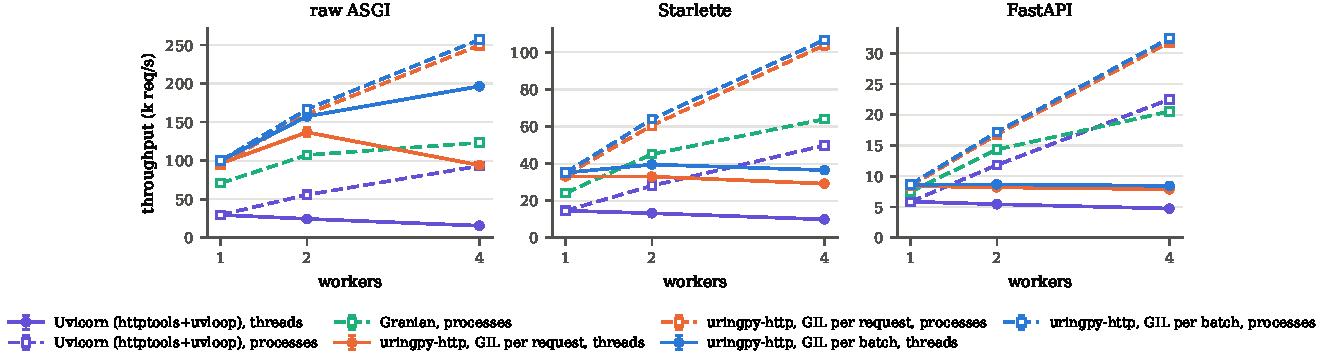
\includegraphics[width=\textwidth]{figures/fig_throughput.pdf}
\caption{Throughput against workers (closed loop, GIL build). Solid lines and filled markers are threads of one interpreter; dashed lines and hollow markers are processes. Error bars are 95\% intervals (most are smaller than the markers).}
\label{fig:tput}
\end{figure*}

Worker threads tell a different story. Uvicorn's threads deliver less with
four workers than with one on every application ($S_4$ = 0.53, 0.68, 0.81),
and each request costs 4.3--4.6 voluntary context switches. Taking the GIL
once per request does not rescue \code{uringpy-http} either. Its four
threads reach 0.98 of one thread on the raw application, with 1.1 context
switches and 0.18 GIL owner changes per request. Batching cuts those to 0.02
and 0.02 and doubles throughput, to 196.5k (2.09\kx{} the per-request mode).
That is 0.76 of four processes. We expected at least 0.90, so that
expectation is refuted. On the frameworks, batching adds 25\% (Starlette) and
7\% (FastAPI) over taking the GIL per request, and the threads stay at 0.34
and 0.26 of processes. Latency follows: at four workers the 99th percentile
of FastAPI requests is 2.4\,s on Uvicorn threads, 238\,ms on batched
\code{uringpy-http} threads and 14\,ms on its processes.

\begin{table}[t]
\caption{Four workers (closed loop, GIL build): threads over processes of the same server (T/P), and per request the voluntary context switches (c.sw.) and GIL owner changes ($g$) of the threads.}
\label{tab:scale}
\centering\footnotesize
\begin{tabular}{@{}llccc@{}}
\toprule
app & server (threads) & T/P & c.sw. & $g$\\
\midrule
raw & Uvicorn, httptools & 0.17 & 4.33 & 0.352\\
 & uringpy-http, GIL/request & 0.38 & 1.11 & 0.180\\
 & uringpy-http, GIL/batch & \textbf{0.76} & 0.021 & 0.020\\
 & uringpy-http, no Python & 1.00 & 0.000 & 0.000\\
\midrule
Starlette & Uvicorn, httptools & 0.20 & 4.40 & 0.432\\
 & uringpy-http, GIL/request & 0.28 & 1.03 & 0.028\\
 & uringpy-http, GIL/batch & 0.34 & 0.021 & 0.020\\
\midrule
FastAPI & Uvicorn, httptools & 0.21 & 4.59 & 0.729\\
 & uringpy-http, GIL/request & 0.25 & 1.01 & 0.024\\
 & uringpy-http, GIL/batch & 0.26 & 0.104 & 0.032\\
\bottomrule
\end{tabular}
\end{table}

\subsection{Time under the GIL (Q3)}

Why do the frameworks gain so little? With timing turned on, one worker of
\code{uringpy-http} holds the GIL for 2.44\,\textmu s per request on the raw
application, 20.8\,\textmu s on Starlette and 105.6\,\textmu s on FastAPI
(Table~\ref{tab:hold}). That is building the scope, the framework's routing
and validation, serialising the response and stepping the coroutine. No
number of threads can exceed $1/t_p$ requests per second, and those
ceilings are 410k, 48.1k and 9.5k. Batched threads reach 0.48, 0.76 and 0.89
of them. For a framework, the GIL is close to saturated, so the remaining
gain from batching, or from anything else done outside the GIL, has to be
small: four FastAPI threads would deliver at most 9.5k/s if hand-offs cost
nothing, against the 8.4k measured. For the raw application the ceiling is
far off, and the 0.76 of processes is limited by something other than
$t_p$. At four threads the raw application's hold time rises to
4.5\,\textmu s, which we attribute to contention for the shared interpreter
state. That is close to the 4\,\textmu s handler at which the earlier
study's batched threads fell to 0.63 of processes.

\begin{table}[t]
\caption{GIL hold per request with one worker, the ceiling it sets on any number of threads, and what four batched threads deliver.}
\label{tab:hold}
\centering\footnotesize
\begin{tabular}{@{}lcccc@{}}
\toprule
app & $t_p$ (\textmu s) & $1/t_p$ (k/s) & 4 threads (k/s) & share\\
\midrule
raw ASGI & 2.44 & 410 & 196.5 & 0.48\\
Starlette & 20.8 & 48.1 & 36.5 & 0.76\\
FastAPI & 105.6 & 9.47 & 8.4 & 0.89\\
\bottomrule
\end{tabular}
\par\smallskip\raggedright\scriptsize Per-request mode gives 2.56, 21.9 and 106.5\,\textmu s. With batching at four threads the timer brackets a whole batch in wall time, and CPython makes the holder drop the GIL every 5\,ms when another thread waits, so batched $t_p$ at $N>1$ overstates the hold (FastAPI: 248\,\textmu s, an impossible utilisation of 2.06); we do not use it.
\end{table}

\subsection{The free-threaded build (Q4)}

Without the GIL, worker threads scale like processes
(Table~\ref{tab:ft}). The interpreter reported the GIL disabled in all 100
server runs. Four batched threads deliver 236.7k on the raw application and
22.3k on FastAPI. That is 0.97 and 0.84 of free-threaded processes, and
1.20\kx{} and 2.65\kx{} what the same threads deliver on the GIL build.
Whether the GIL is taken per batch or per request no longer matters (within
2--4\%). The FastAPI result is below the 0.90 we expected, so that part of
the expectation is refuted. A single worker pays for the build: 4\% on the
raw application and 17\% on FastAPI. Four free-threaded processes deliver
0.82 of the GIL build's processes on FastAPI. Uvicorn's threads also scale
on this build (0.91 and 0.87 of its processes), but they start from a
lower point.

\begin{table}[t]
\caption{Free-threaded CPython~3.14.8t: thousands of requests per second and threads over processes at four workers.}
\label{tab:ft}
\centering\footnotesize
\begin{tabular}{@{}llccc@{}}
\toprule
app & server & $N$=1 & $N$=4 & T/P\\
\midrule
raw & uringpy-http, GIL/batch & 95.8 & 236.7 & 0.97\\
 & uringpy-http, GIL/request & 91.1 & 232.3 & 0.95\\
 & Uvicorn, httptools+asyncio & 24.4 & 68.1 & 0.91\\
\midrule
FastAPI & uringpy-http, GIL/batch & 7.1 & 22.3 & 0.84\\
 & uringpy-http, GIL/request & 6.9 & 21.5 & 0.81\\
 & Uvicorn, httptools+asyncio & 4.9 & 16.3 & 0.87\\
\bottomrule
\end{tabular}
\par\smallskip\raggedright\scriptsize \code{uvloop} is not available for this build. Processes: raw 244.6 and 75.2; FastAPI 26.5 and 18.8.
\end{table}

\subsection{Open-loop latency}

Figure~\ref{fig:ol} shows tail latency under fixed offered rates with four
workers. On the raw application, batched \code{uringpy-http} processes keep
the 99th percentile under 4\,ms up to 200k~requests/s (median 1.61\,ms). Up
to 50k~requests/s Uvicorn's processes are as fast as the other
configurations, but they cannot keep up at 100k. Batched threads keep up to
200k, at a 99th percentile of 0.85\,s, and fall behind at 250k. Threads that
take the GIL per request fall behind at 100k. On FastAPI, Uvicorn's
processes keep up with 20k~requests/s, but their 99th percentile reaches
2.0\,s. Batched \code{uringpy-http} processes serve the same rate at 5.7\,ms,
keep up with 30k, and fall behind at 40k. Threads on FastAPI cannot keep up
even with 10k, because that is more than their closed-loop capacity of
8.4k.

\begin{figure*}[t]
\centering
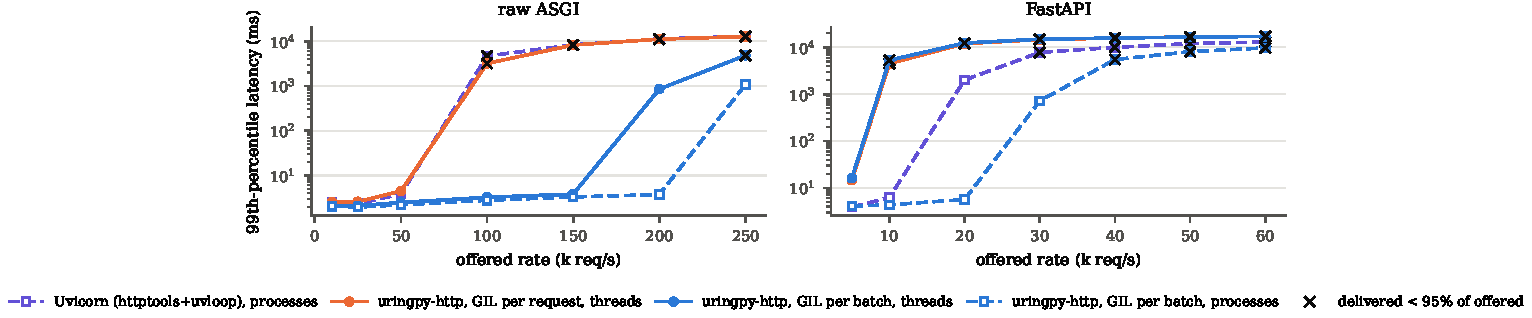
\includegraphics[width=\textwidth]{figures/fig_openloop.pdf}
\caption{99th-percentile latency under open-loop load (wrk2, corrected for coordinated omission), four workers, log scale. A cross marks a run that delivered less than 95\% of the offered rate.}
\label{fig:ol}
\end{figure*}

\subsection{Expectations and outcomes}

Of the fourteen expectations committed before the runs, eleven held. Two
were refuted, both about how close threads come to processes: batched
threads on the raw application (0.76 against $\ge$0.90) and free-threaded
threads on FastAPI (0.84 against $\ge$0.90). One could not be tested:
open-loop median latency at a quarter of capacity for FastAPI, because the
lowest offered rate was already above half the capacity of the thread
configurations. Every per-request speedup over Uvicorn that we predicted
held, with margin. \code{paper/OUTCOMES.md} lists all fourteen.

\section{Discussion}

\textbf{Where the time goes.} A request served by Uvicorn spends most of its
time in the server, not the application. Moving the transport and the
parser out of Python makes the raw application 3.36\kx{} faster, while
FastAPI, which spends about 100\,\textmu s of its own per request, gains
1.47\kx{}. The gain is largest for small, fast endpoints, such as health
checks, proxies and JSON APIs with light validation, and it holds with
processes as well as with one worker.

\textbf{What batching can and cannot do.} Batching attacks the hand-offs
($g$), and it removes nearly all of them: context switches fall from about
one per request to two per hundred. That doubles thread throughput when the
application is cheap. The ceiling $1/t_p$ does not move, though, and real
frameworks sit close to it. On the GIL build, threads are a way to share
memory and connection pools, not a way to use more cores. That holds for
any server, because $t_p$ belongs to the application.

\textbf{Deployment.} On the GIL build, run \code{uringpy-http} with one
process per core. On the free-threaded build, threads are within 3--16\% of
processes and share one interpreter's memory, at a 4--17\% cost per core
that should shrink as the build matures. Threads on the GIL build make
sense only for applications that hold the GIL for a few microseconds.

\section{Threats to Validity}

All runs were on one four-core machine type, in one zone, in one session on
one day. The earlier study saw throughput vary by 0.89--1.09\kx{} between
days, so the absolute numbers carry that uncertainty, though ratios measured
in the same session are less affected. The applications are small and do no
I/O of their own; an application that waits on a database is served by the
worker's loop (Section~III), which these benchmarks exercise only in tests.
The closed-loop runs used 400 connections. Ten runs, all Uvicorn with
FastAPI at one worker, had 32--56 wrk timeouts each in about 117k requests;
their slowest responses exceeded the 10\,s timeout. We kept these runs in
the means. The parser and the transport were not measured separately. Our
server implements a subset of HTTP (Section~III), and a server that
implemented TLS or HTTP/2 would do more work per request. Finally, the
batched GIL timer overstates the hold at more than one thread, as
Table~\ref{tab:hold} notes, so we interpret only the one-worker value.

\section{Conclusion}

Parsing HTTP and driving the socket in C with the GIL released makes a
request through a Python ASGI server 1.47--3.36\kx{} cheaper than through
Uvicorn, and the gain holds at four processes (1.44--2.76\kx{}). Batching
the GIL removes almost every hand-off between worker threads and doubles
their throughput for a light application. It cannot raise the ceiling that
the application's own time under the lock sets. For Starlette and FastAPI
that ceiling is close, so on the GIL build processes remain the way to use
more cores, and on the free-threaded build threads come within 3--16\% of
them.

\textbf{Availability.} Code, tests, raw run files, the scripts that produced
every table and figure, and the expectations recorded before the runs are
at \url{https://github.com/marimuthuvm/uringpy-http} (MIT).

\footnotesize
\begin{thebibliography}{99}
\setlength{\itemsep}{0pt}
\bibitem{uringpy} M.~Velayutham, ``The lock, not the system call: What batching buys multithreaded Python servers under the GIL,'' 2026. Code and data: \url{https://github.com/marimuthuvm/uringpy}, doi:10.5281/zenodo.23262923.
\bibitem{uvicorn} Encode, ``Uvicorn: an ASGI web server,'' \url{https://www.uvicorn.org}.
\bibitem{uvloop} MagicStack, ``uvloop: ultra fast asyncio event loop,'' \url{https://github.com/MagicStack/uvloop}.
\bibitem{llhttp} F.~Indutny et al., ``llhttp: port of http\_parser to llparse,'' \url{https://github.com/nodejs/llhttp}; Python binding \code{httptools}, \url{https://github.com/MagicStack/httptools}.
\bibitem{picohttpparser} K.~Oku et al., ``PicoHTTPParser: a tiny, primitive, fast HTTP request/response parser,'' \url{https://github.com/h2o/picohttpparser}.
\bibitem{h2o} K.~Oku et al., ``H2O: the optimized HTTP/1.x, HTTP/2, HTTP/3 server,'' \url{https://h2o.examp1e.net}.
\bibitem{granian} G.~Barbieri, ``Granian: a Rust HTTP server for Python applications,'' \url{https://github.com/emmett-framework/granian}.
\bibitem{asgi} ``ASGI (Asynchronous Server Gateway Interface) specification,'' version 3.0, HTTP spec 2.4, \url{https://asgi.readthedocs.io}.
\bibitem{starlette} Encode, ``Starlette,'' \url{https://www.starlette.io}.
\bibitem{fastapi} S.~Ram\'irez, ``FastAPI,'' \url{https://fastapi.tiangolo.com}.
\bibitem{axboe} J.~Axboe, ``Efficient IO with io\_uring,'' 2019, \url{https://kernel.dk/io_uring.pdf}.
\bibitem{beazley} D.~Beazley, ``Understanding the Python GIL,'' PyCon, 2010.
\bibitem{amdahl} G.~M. Amdahl, ``Validity of the single processor approach to achieving large scale computing capabilities,'' in \emph{Proc.\ AFIPS Spring Joint Computer Conf.}, 1967, pp.~483--485.
\bibitem{eyerman} S.~Eyerman and L.~Eeckhout, ``Modeling critical sections in Amdahl's law and its implications for multicore design,'' in \emph{Proc.\ ISCA}, 2010, pp.~362--370.
\bibitem{pep703} S.~Gross, ``PEP 703: Making the Global Interpreter Lock optional in CPython,'' 2023, \url{https://peps.python.org/pep-0703/}.
\bibitem{wrk2} G.~Tene, ``wrk2: a constant throughput, correct latency recording variant of wrk,'' \url{https://github.com/giltene/wrk2}.
\end{thebibliography}

\end{document}
